%%
%% This is file `sample__1col_minted.tex',
%% generated with the docstrip utility.
%%
%% The original source files were:
%%
%% sample.dtx  (with options: `all,1col,minted')
%% -------:| -----------------------------------------------------------------
%%  sample:| The sample document for CEURART class
%%  Author:| Dmitry S. Kulyabov, Ilaria Tiddi, Manfred Jeusfeld
%%  E-mail:| kulyabov-ds@rudn.ru, i.tiddi@vu.nl, Manfred.Jeusfeld@acm.org
%% License:| Released under the Creative Commons License Attribution 4.0 International (CC BY 4.0)
%%     See:| https://creativecommons.org/licenses/by/4.0/deed.en
%%
%% The first command in your LaTeX source must be the \documentclass command.
%%
%% Options:
%% twocolumn : Two column layout. Do not use twocolumn for papers submitted to CEUR-WS!
%% hf: enable header and footer.
% \documentclass[%
% ]{ceurart}
\documentclass[twocolumn]{ceurart}

%%
%% One can fix some overfulls
\sloppy

%% Minted listings support
%% Need pygment <http://pygments.org/> <http://pypi.python.org/pypi/Pygments>
\usepackage{minted}
%% auto break lines
\setminted{breaklines=true}

%% end of the preamble, start of the body of the document source.
\begin{document}

%%
%% Rights management information.
%% CC-BY is default license.
\copyrightyear{2025}
\copyrightclause{Copyright for this paper by its authors.
Use permitted under Creative Commons License Attribution 4.0 International (CC BY 4.0).}

%%
%% This command is for the conference information
\conference{
   ANSyA 2025: $1^{st}$ International Workshop on Advanced Neuro-Symbolic Applications,
   co-located with ECAI 2025.
}

%%
%% The "title" command
\title{A Challenging Dataset of Jet Engine Fault Scenarios}


%%
%% The "author" command and its associated commands are used to define
%% the authors and their affiliations.
\author[1]{Christoforos Romesis}[%
orcid=0009-0001-6485-5548,
email=chris.romesis@iit.demokritos.gr,
url=https://github.com/data-eng,
]
\cormark[1]
\fnmark[1]

\author[1]{Stasinos Konstantopoulos}[%
orcid=0000-0002-2586-1726,
email=konstant@iit.demokritos.gr,
url=https://github.com/data-eng,
]
\fnmark[1]

\address[1]{Institute of Informatics and Telecommunications, NCSR Demokritos,
  Patr.Gregoriou E \& 27 Neapoleos Str, 15341 Agia Paraskevi, Greece}

%% Footnotes
\cortext[1]{Corresponding author.}
\fntext[1]{These authors contributed equally.}

%%
%% The abstract is a short summary of the work to be presented in the
%% article.
\begin{abstract}
  This dataset description paper introduces a challenging sequence
  processing task. Specifically, the task is to recognize faults from
  aircraft gas turbine engine conditions where previous faults
  determine how the presently observed conditions should be
  interpreted. Several state-of-the-art deep-learning sequence
  processors have been tested on the task, and these preliminary
  results demonstrate that they cannot correctly model the phenomenon.
\end{abstract}

%%
%% Keywords. The author(s) should pick words that accurately describe
%% the work being presented. Separate the keywords with commas.
\begin{keywords}
  time-series dataset \sep
  sequence processing \sep
  long-range dependencies \sep
  gas turbine faults 
\end{keywords}

%%
%% This command processes the author and affiliation and title
%% information and builds the first part of the formatted document.
\maketitle

\section{Motivation and Purpose}

Time series forecasting and time series classification are the major
\emph{sequence processing} tasks, and both depend on a method's
ability to identify time-based patterns in the data. When dealing
with \emph{long sequence} processing in particular, successful methods
must identify non-local patterns such as trends, seasonality, and
long-range dependencies. Observing large-scale and high-impact
repositories such as the 
\emph{Monash Time Series Forecasting Archive} \citep{godahewa-etal-2021}
reveals an abundance of datasets that exhibit long-term trends and
long-period seasonal patterns, but a lack of datasets that exhibit
non-periodic long-range dependencies. Unsurprizingly, successful
methods stem from the non-parametric statistics field or from the deep
learning field.

The sequential integration of sub-symbolic and symbolic modules allows
connectionist recognition of single events to interact with long-range
dependencies between events. Such \emph{neuro-symbolic} approaches are
powerful, but to demonstrate their effectiveness they must be applied
to datasets and tasks where the following conditions hold simultaneously:
(a) the recognition of individual events in the raw data is a
non-trivial pattern recognition task for which connectionist methods
are more appropriate; and (b) this recognition is affected by unknown
symbolic patterns that need to be discovered in conjunction with the
sub-symbolic patterns themselves.

In this dataset description paper we present such a task where purely
connectionist sequence processing performs substantially below the par
established through the usual trend and seasonality tasks and where
neuro-symbolic methods can demonstrate their effectiveness in
challenging real-world applications.

\section{Dataset Description}

Jet engines play a vital role in aviation, and ensuring their safety and reliability is paramount. The harsh environments they operate in can cause malfunctions, impacting aerothermodynamic measurements. Detecting faults in-flight from time-series data remains challenging due to limited instrumentation, similar fault effects, concurrent faults, and prior events. This paper introduces a dataset of simulated time-series measurements from a turbofan engine, including various common faults, to aid in developing fault detection strategies. This dataset is valuable for the Machine Learning community, presenting a complex engineering problem with unique features. It includes 2{,}410 time series, each with 3{,}600 time steps, where faults are introduced, and measurements are taken at every step. Some faults have nearly indistinguishable effects, posing challenges for differentiation, while others exhibit long-term dependencies. These attributes make the dataset suitable for research in sequential and time-stepwise classification and investigating long-term dependencies. The dataset comprises time series measurements from a low bypass ratio turbofan engine, typical of modern civil aviation engines, generated using an Engine Performance Model.
The dataset has been archived and is publicly accessible from \url{https://doi.org/10.5281/zenodo.15856441}


\subsection{Engine Performance Model}

An EPM interrelates parameters that represent engine component health and operating conditions with measurements performed on an engine \citep{alexiou_development_2005}, and can be expressed through Equation~(\ref{eq:epm}):

\begin{eqnarray}\label{eq:epm}
\mathbf{Y} = \mathbf{g}(\mathbf{u}, \mathbf{f})
\end{eqnarray}
%
where $\mathbf{g}$ is a vector function representing the EPM, $\mathbf{u}$ is a vector of measured 
quantities defining the engine's operating point, $\mathbf{Y}$ is a set of measurements for condition monitoring, and $\mathbf{f}$ is a vector of engine component \textit{health parameters}. Typically, two health parameters are used for each component: the flow factor (SW), indicating the component's swallowing capacity, and the efficiency factor (SE), representing thermal efficiency. The application of such parameters for assessing engine component health has been discussed in \citep{mathioudakis_performance_2001}. A deviation of a health parameter from its nominal value signals a fault in that component. As extensively discussed in \citep{mathioudakis_signatures_2024} the ratio of deviations between two health parameters can serve as a characteristic metric for faults such as fouling, increased tip clearance, erosion, and foreign object damage. The severity of the fault correlates with the level of this deviation. The deviation (or \textit{delta}) of a health parameter $\mathbf{\Delta f}$ is defined as:

\begin{eqnarray}\label{eq:deltaf}
    \mathbf{\Delta f}\ (\%) = \frac{\mathbf{f} - \mathbf{f_o}}{\mathbf{f_o}} \cdot 100\%
\end{eqnarray}
%
where $\mathbf{f}$ denotes the value of the health parameter, and $\mathbf{f_o}$ its nominal value.

Using the EPM, the nominal values of the available measurement set, denoted as $\mathbf{Y_o}$, 
can be computed for a specified operating point $\mathbf{u}$. These values correspond to the nominal health parameters, $\mathbf{f_o}$, and are derived via the following relation:

\begin{eqnarray}\label{eq:epmnom}
\mathbf{Y_o} = \mathbf{g}(\mathbf{u}, \mathbf{f_o})
\end{eqnarray}

Once a measurement vector $\mathbf{Y}$ is obtained from the engine, the relative deviation $\mathbf{\Delta Y(\%)}$
from its nominal value $\mathbf{Y_o}$ is defined as:

\begin{eqnarray}\label{eq:deltay}
    \mathbf{\Delta Y}(\%) = \frac{\mathbf{Y} - \mathbf{Y_o}}{\mathbf{Y_o}} \cdot 100\%
\end{eqnarray}

To emulate realistic measurement conditions, random noise is superimposed on the measurement 
deviations. The noise levels considered are consistent with those typical of this instrumentation, 
as documented in \citep{romesis_model-assisted_2024}.

\subsection{Dataset Generation}

The EPM used for dataset generation was developed in MATLAB. At each time step, the data includes a labeled vector of measurement deltas produced by the EPM at a specified operating point and a specific engine health condition. A total of 10 operating points were considered, covering a broad range of the engine’s flight envelope. Throughout a time series, all time steps correspond to the same operating point. Additionally, five distinct health conditions were considered, as summarized in Table~\ref{tab:health_conditions}. The first health condition represents the nominal, healthy operation of the engine. The second health condition (coded as TIP) models an increased clearance of the compressor blades. As reported in \citep{mathioudakis_signatures_2024}, this fault results in a ratio of the related health parameter deviations, $\Delta SW/\Delta SE$, of $0.2$; the actual deviations of $\Delta SW$ and $\Delta SE$ are around $-1\%$ and $-5\%$, respectively. The remaining three conditions involve a mistuning of the inlet guide vanes of the compressor, damage caused by foreign objects within the compressor, and the concurrent occurrence of VGV and FOD faults. These conditions result in a ratio of $-3$, $1$, and $0.2$, respectively. In all cases, deviations within the range of $0.7$ to $1.3$ times the aforementioned values are considered, simulating faults of varying severity. Notably, the effects of TIP faults and the combined VGV+FOD faults on the compressor’s health parameters are the same, and therefore, measurements under these conditions follow the same distribution. Each dataset record is labeled according to the specific health condition present at that time step.

\begin{table}[h]
% \begin{table}
\caption{Considered health conditions.}
\label{tab:health_conditions}
\centering
\begin{tabular}{ccccc} 
\toprule
label &  health condition & $\Delta SW$ & $\Delta SE$ & $\Delta SW/\Delta SE$ \\
\midrule
1	& Healthy	& 0\%	& 0\%	& N/A \\
2	& TIP fault	& -1\%	& -5\%	& 0.2 \\
3	& VGV fault	& +3\%	& -1\%	& -3 \\
4	& FOD fault	& -4\%	& -4\%	& 1 \\
5	& VGV+FOD faults	& -1\%	& -5\%	& 0.2 \\
\bottomrule
\end{tabular}
\end{table}

Each time series comprises 3{,}600 time steps. During this period, various health conditions may develop. A time series without any fault contains measurements indicative of healthy engine operation at all time steps. In other time series, the engine operates fault-free initially, but at a certain point, a TIP, VGV, or FOD fault occurs and persists until the end of the series. In some other time series, the engine also operates fault-free initially, but at a certain point, a brief period occurs during which a VGV fault is present. The engine then continues to operate without faults until a later time step, when a combined VGV+FOD fault manifests and persists for the remainder of the time series. This scenario exemplifies a specific fault condition characterized by a severe VGV fault leading to FOD. The damage is attributed to the detachment of a particle from the VGV mechanism, such as a loosened bolt, which is subsequently ingested by the engine. The failure of the VGV mechanism may be preceded by a transient VGV fault event, serving as an early indicator of the impending failure. This scenario was selected because both the TIP and VGV+FOD faults exert similar impacts on engine performance. The key differentiator between the TIP fault and the VGV+FOD fault is the long-term dependency of the latter on the initial, instantaneous VGV fault.

\section{Concluding Remarks and Next Steps}

The dataset is used to evaluate the classification capabilities of sequential machine learning methods on time-series data with long-term dependencies. Preliminary results suggest the dataset challenges current techniques. For example, Figure~\ref{fig:results} shows four classification methods trained on the dataset and tested on a time-series segment containing a VGV+FOD fault. The methods, include an RNN, a GRU, and an LSTM, together with an MLP, trained for point-to-point classification for comparison. All methods failed to detect the VGV+FOD fault, though they detected a precursor VGV fault at time step 740. Sequential methods have shown limited ability to use information from prior time steps, performing similarly to the point-wise MLP.

\begin{figure}[h]
  \centering
  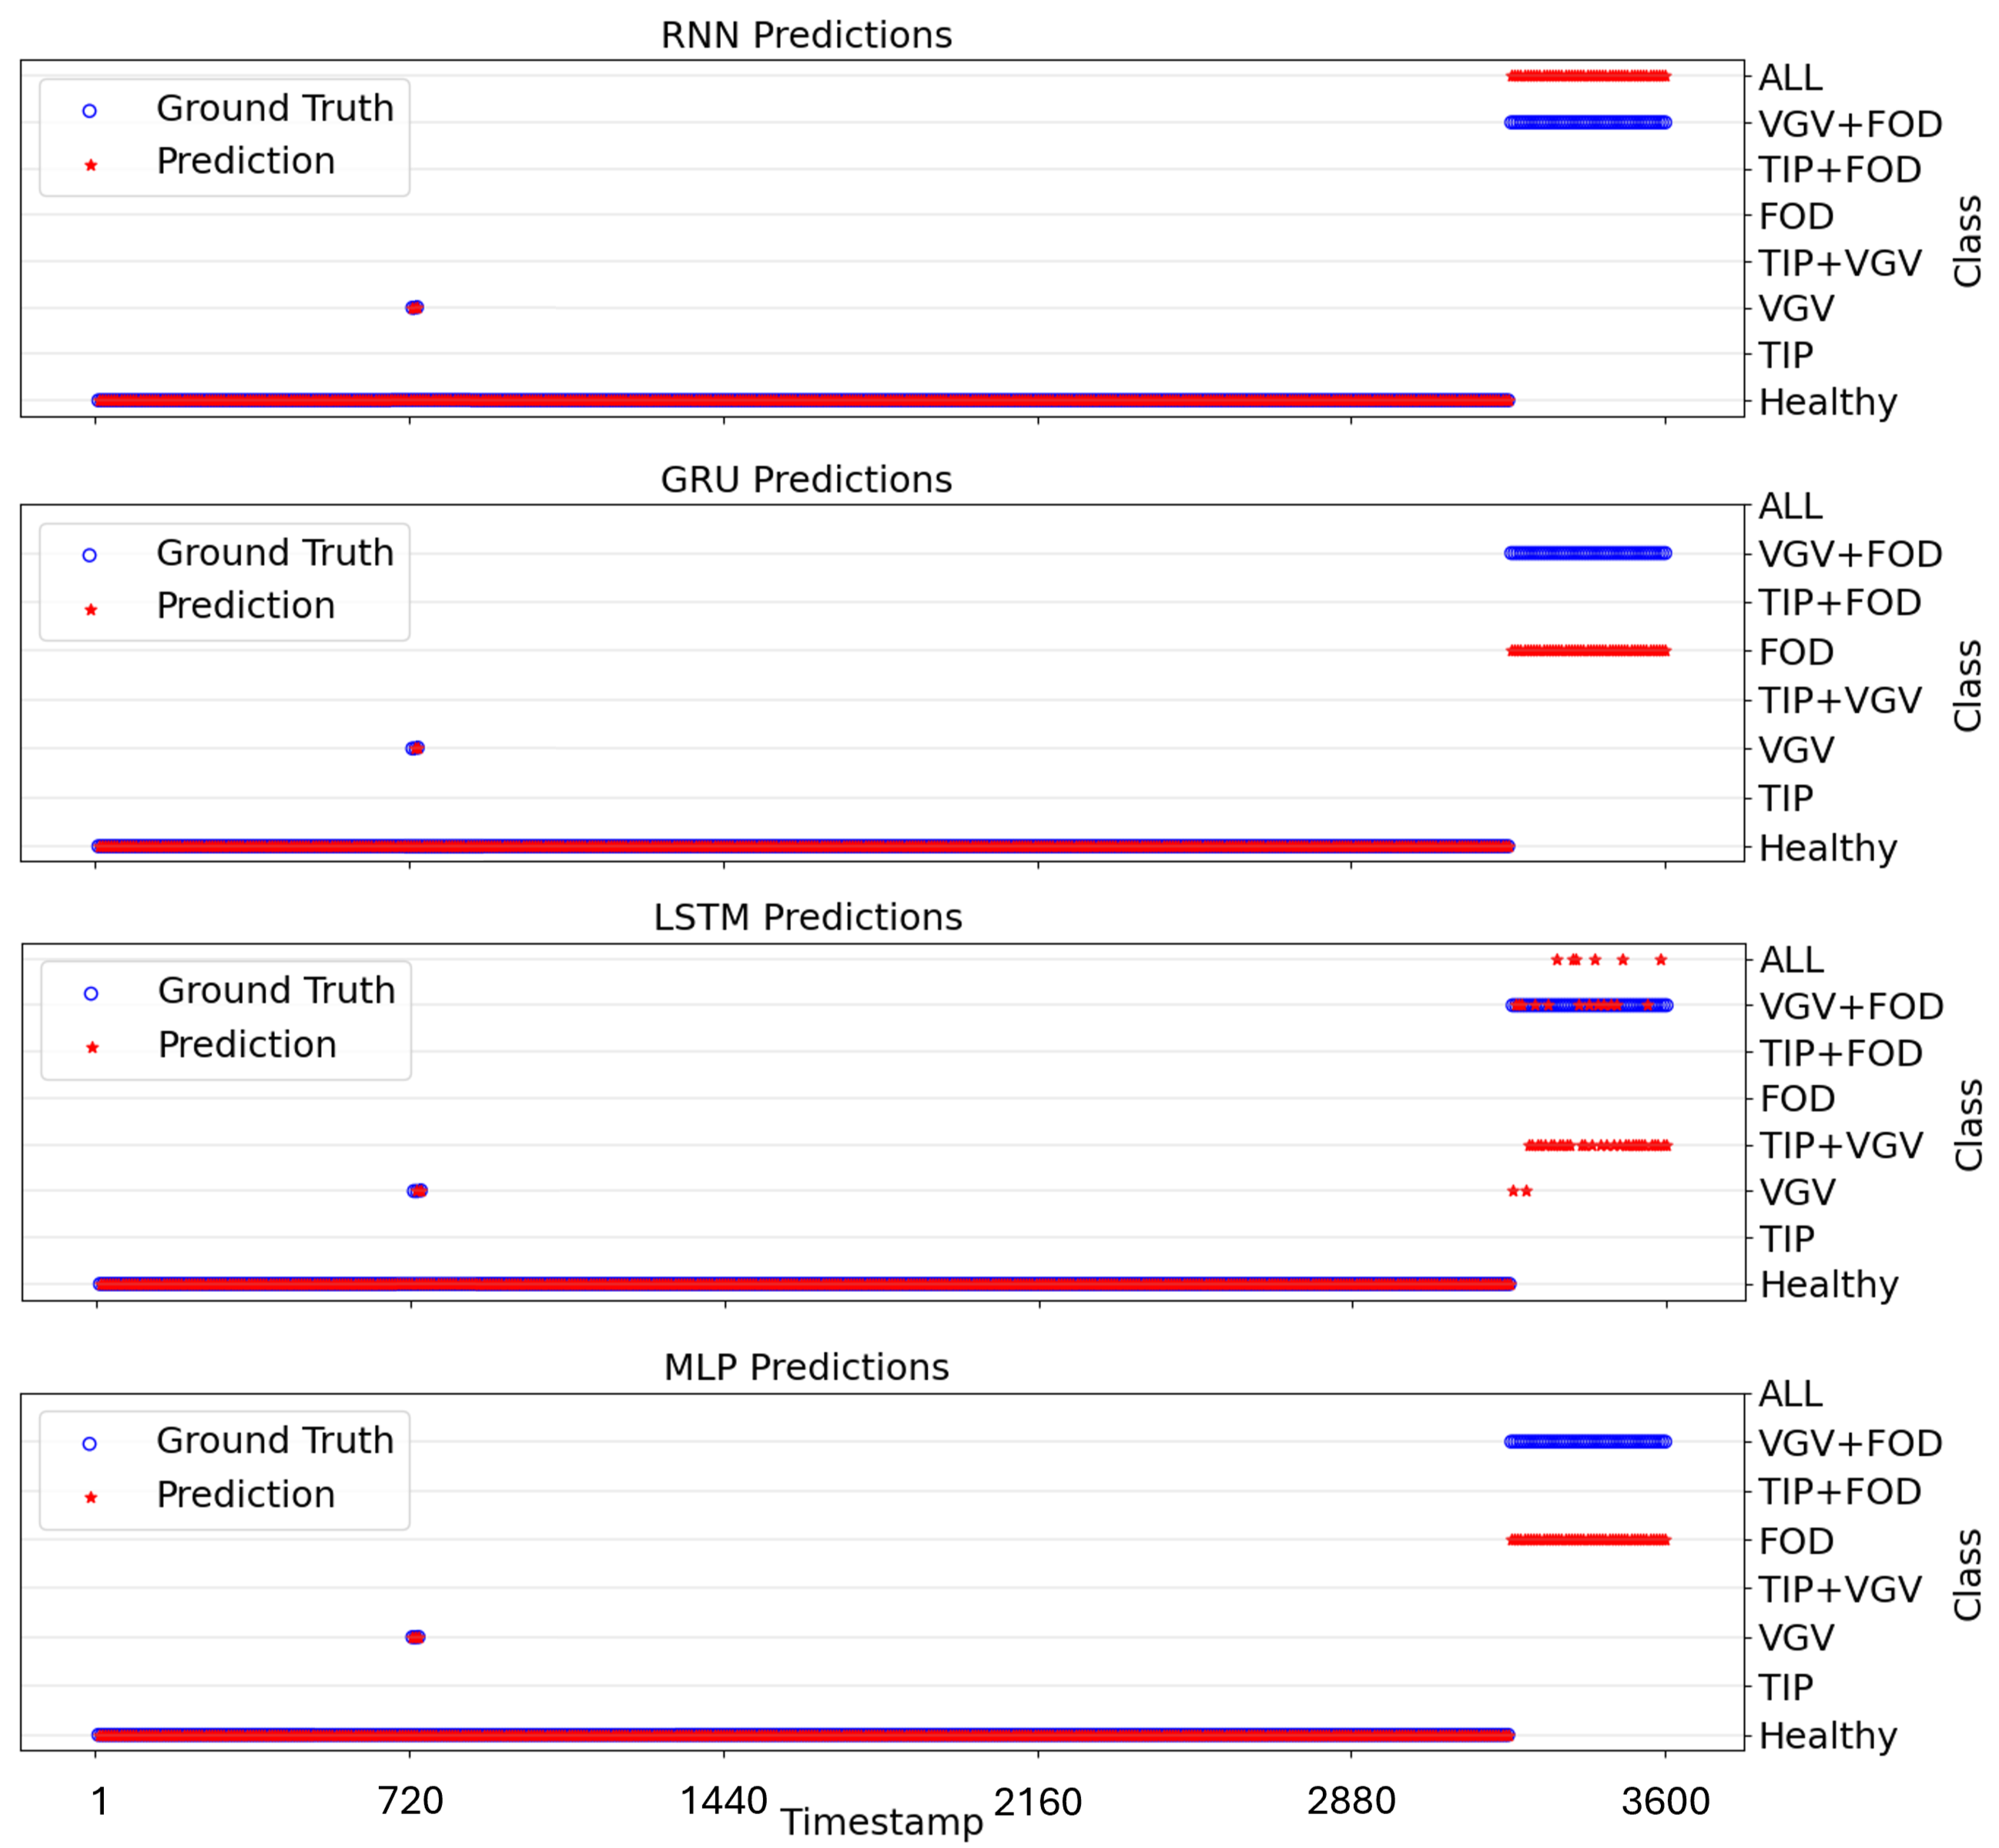
\includegraphics[width=\linewidth]{comparison_eval_tsid_8_demo}
  \caption{Health conditions detection during a time-series of the dataset.}
  \label{fig:results}
\end{figure}


%% The acknowledgments section is defined using the "acknowledgments" environment
%% (and NOT an unnumbered section). This ensures the proper
%% identification of the section in the article metadata, and the
%% consistent spelling of the heading.
\begin{acknowledgments}
This research was co-funded by the European Union under GA no. 101135782 (MANOLO project). Views and opinions expressed are however those of the authors only and do not necessarily reflect those of the European Union or CNECT. Neither the European Union nor CNECT can be held responsible for them.
\end{acknowledgments}

\begin{aideclaration}
    The authors have not employed any Generative AI tools.
\end{aideclaration}

%%
%% Define the bibliography file to be used
% \bibliography{sample-ceur}
\bibliography{mybibfile}

%%
%% If your work has an appendix, this is the place to put it.


\end{document}
%%% Local Variables:
%%% mode: LaTeX
%%% TeX-master: t
%%% End:
%% This work consists of the file sample.dtx and a Makefile.
%% Running "make" generates the derived files README, sample*.tex, and sample*.pdf.
%% Running "make userinstall" installs the files in the user's TeX tree.
%% Running "make install" installs the files in the local TeX tree.
%%
%% End of file `sample__1col_minted.tex'.
